% Figure snippets for main.tex. All values trace to experimental_log.md.

\begin{figure}[htbp]
\centering
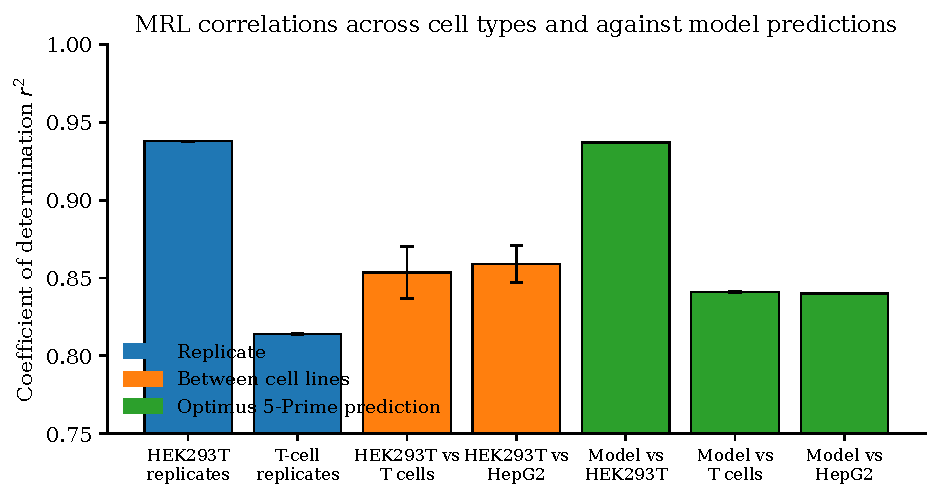
\includegraphics[width=0.88\textwidth]{figures/fig1_cross_cell_r2.pdf}
\caption{Mean ribosome load (MRL) is highly reproducible across replicates
and highly correlated across cell types, and the HEK293T-trained model
transfers to both T cells and HepG2. Replicate $r^{2}$ values are 0.938
(HEK293T) and 0.814 (T cells). Between-cell-line $r^{2}$ ranges are
0.837--0.870 (HEK293T vs T cells) and 0.847--0.871 (HEK293T vs HepG2);
error bars show the extreme values of these ranges. The HEK293T-trained
Optimus 5-Prime model achieves $r^{2} = 0.937$ on held-out HEK293T data,
$r^{2} = 0.841$ on T cells, and $r^{2} = 0.840$ on HepG2.}
\label{fig:cross_cell}
\end{figure}

\begin{figure}[htbp]
\centering
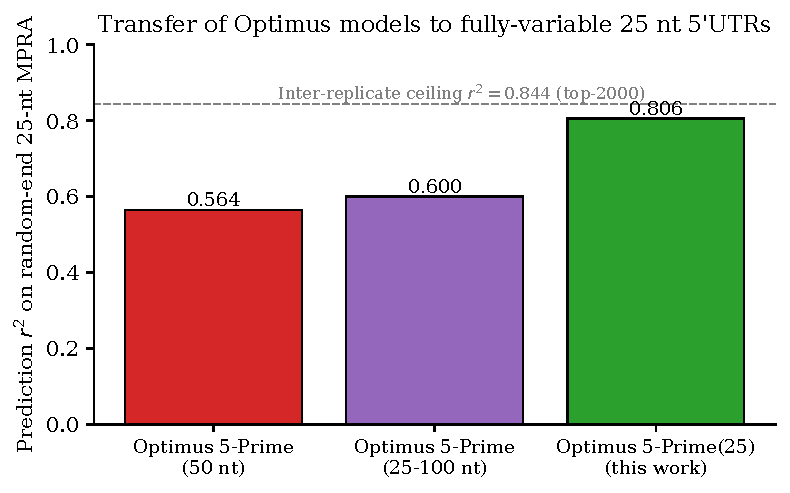
\includegraphics[width=0.78\textwidth]{figures/fig2_model_r2_25nt.pdf}
\caption{Previously developed Optimus 5-Prime models trained on
fixed-end libraries transfer poorly to the random-end 25~nt 5'UTR
library ($r^{2} = 0.564$ for the 50~nt model; $r^{2} = 0.600$ for the
25--100~nt model), whereas a model retrained on the random-end 25~nt
data (Optimus 5-Prime(25)) reaches $r^{2} = 0.806$ on a held-out test
set, close to the inter-replicate ceiling of $r^{2} = 0.844$ estimated
on the top-2000 sequences by read coverage.}
\label{fig:model_25nt}
\end{figure}

\begin{figure}[htbp]
\centering
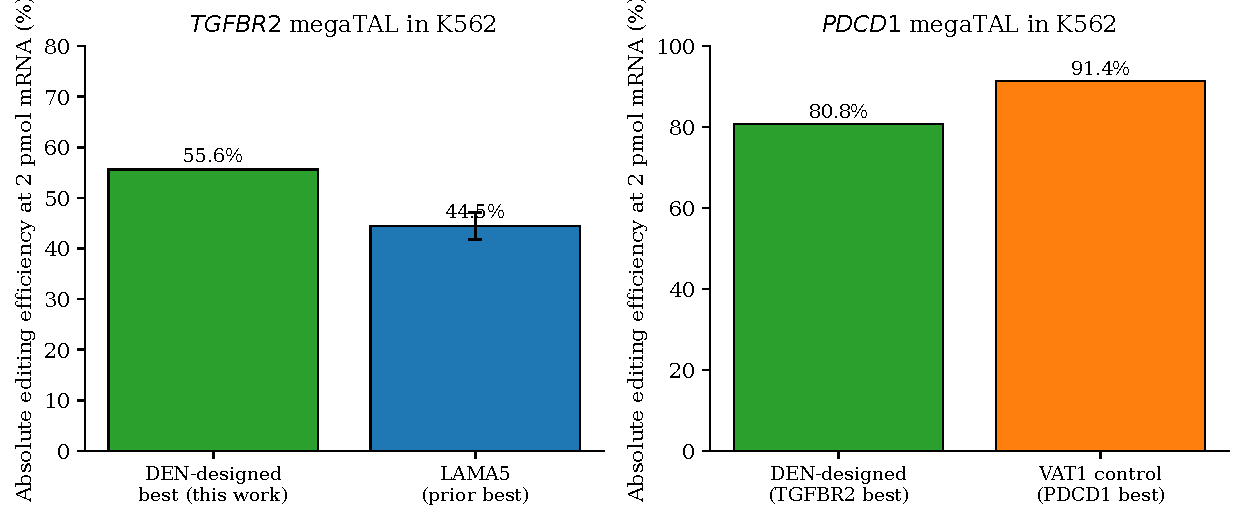
\includegraphics[width=0.95\textwidth]{figures/fig3_editing_efficiency.pdf}
\caption{Absolute gene editing efficiency at 2~pmol mRNA in K562 cells.
\textbf{Left:} targeting \emph{TGFBR2}, the best DEN-designed 5'UTR
reaches 55.6\% editing, an 18--33\% improvement over the previous best
natural control LAMA5 (gray bar shows the implied LAMA5 range).
\textbf{Right:} for the same \emph{PDCD1} megaTAL cargo, the DEN-designed
5'UTR that was best on \emph{TGFBR2} yields only 80.8\% editing
(comparable to a Strong Kozak control), while the VAT1 natural control
is best at 91.4\%. This cargo-specific ordering illustrates that the
highest-MRL 5'UTR is not always the highest-editing 5'UTR.}
\label{fig:editing}
\end{figure}

\begin{figure}[htbp]
\centering
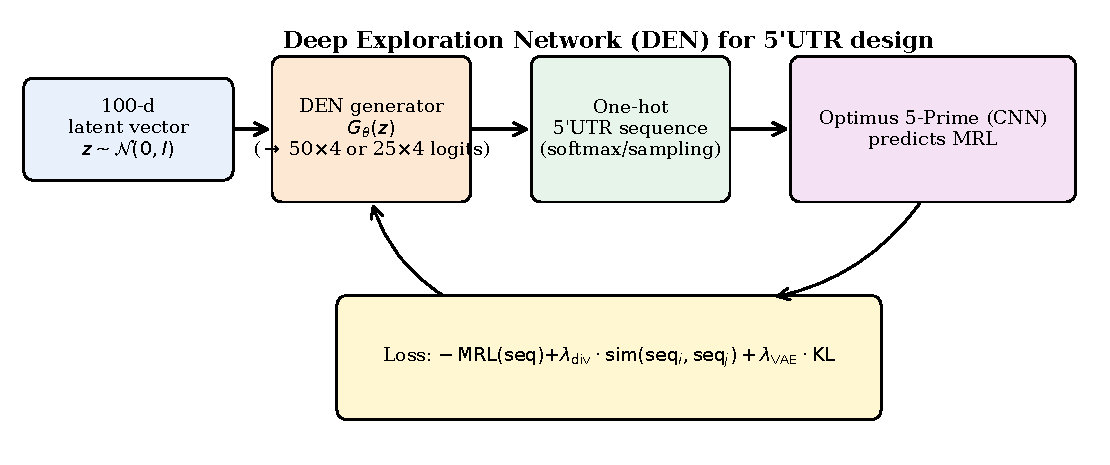
\includegraphics[width=0.95\textwidth]{figures/fig4_den_schematic.pdf}
\caption{Schematic of the Deep Exploration Network (DEN) 5'UTR design
pipeline used in this work. A 100-dimensional latent vector is mapped
by the generator $G_\theta$ to a 50$\times$4 or 25$\times$4 one-hot
sequence logit; the sampled sequence is scored by a CNN MRL predictor
(Optimus 5-Prime or Optimus 5-Prime(25)); training minimizes negative
predicted MRL plus a pairwise similarity penalty and an optional VAE
regularizer to keep generated sequences in-distribution.}
\label{fig:den_schematic}
\end{figure}
